\documentclass{article}
\usepackage[margin=2cm]{geometry}
\hyphenpenalty=10000
\usepackage{graphicx}

\begin{document}
\title{MXB262 Case Studies Part A}
\author{Braydan Newman n11272031}
\date{}
\maketitle

\pagebreak 

\tableofcontents{}

\pagebreak 

\section{Visualizations Descriptions}
\subsubsection{Visualization 1}
\begin{figure}[!htb]
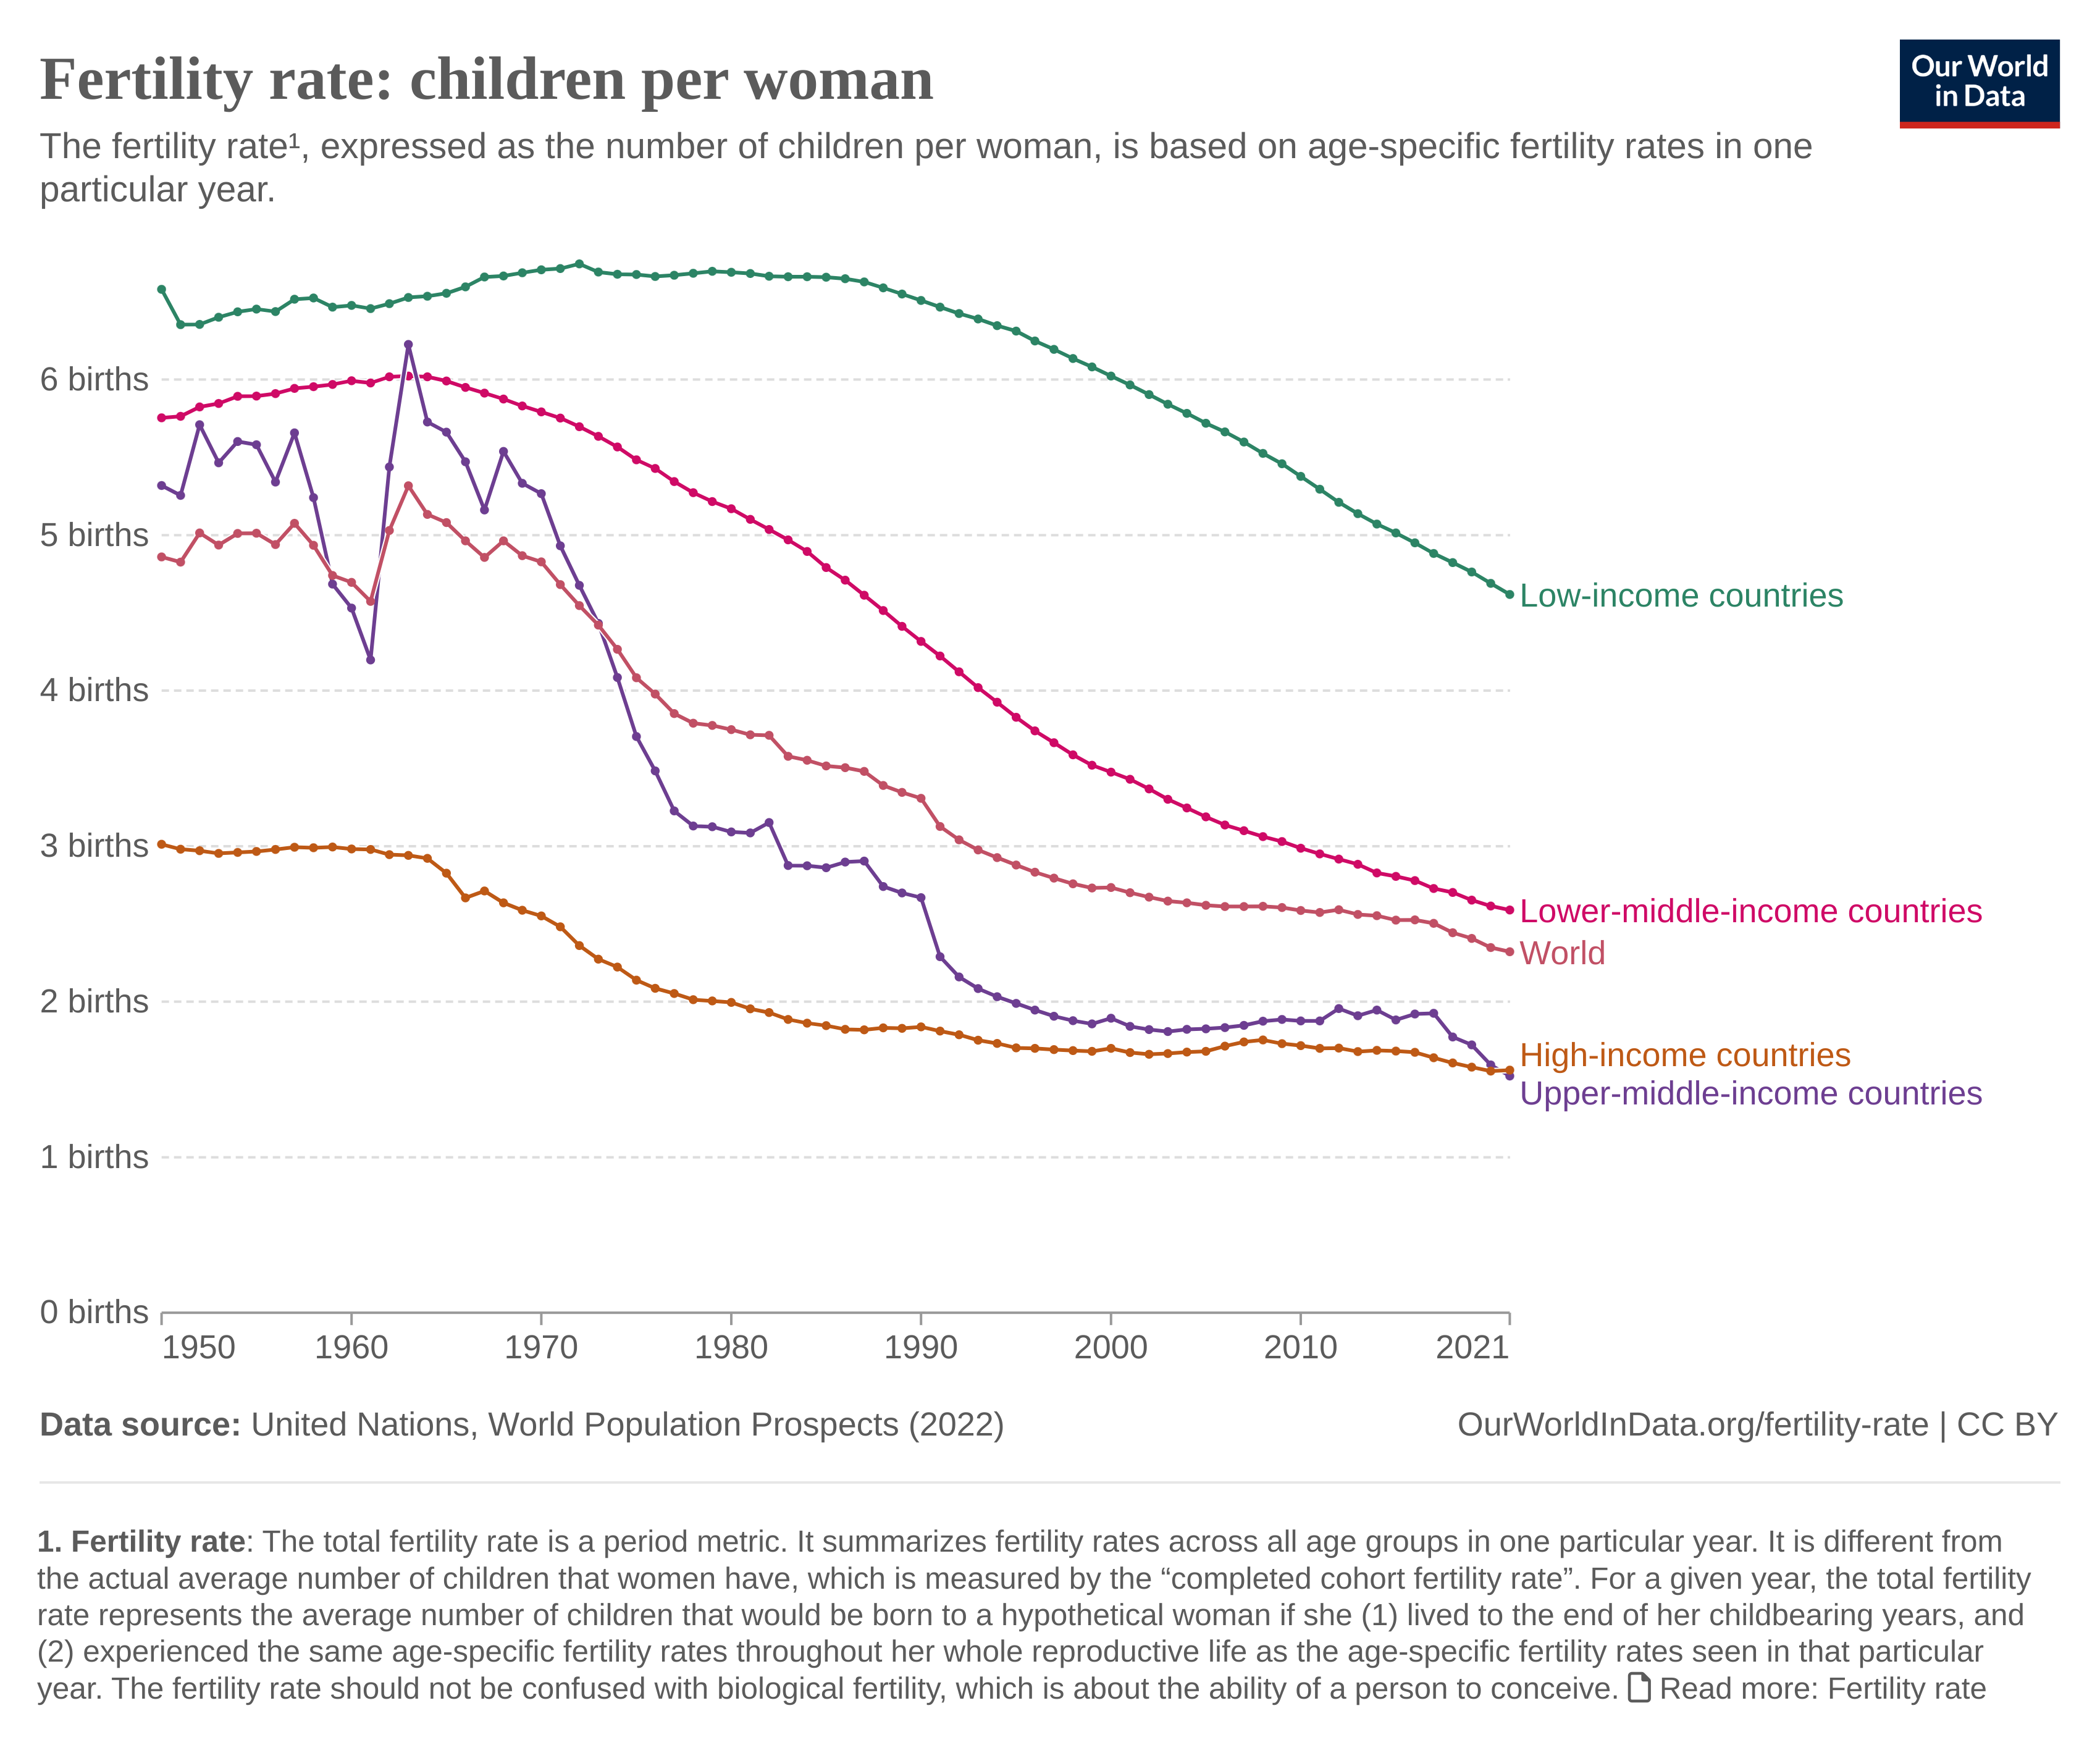
\includegraphics[width=\textwidth]{children-per-woman-un (1).png} 
\caption{World Fertility Rate (Source: https://ourworldindata.org/fertility-rate )}

\end{figure}

The above graph is a line graph showing the Fertility Rate from the years 1950 to 2021. This Graph displays the fertility rate by Children Per Women with different lines representing countries in addition to different income brackets.

\pagebreak 

\subsubsection{Visualization 2}
\begin{figure}[!htb]
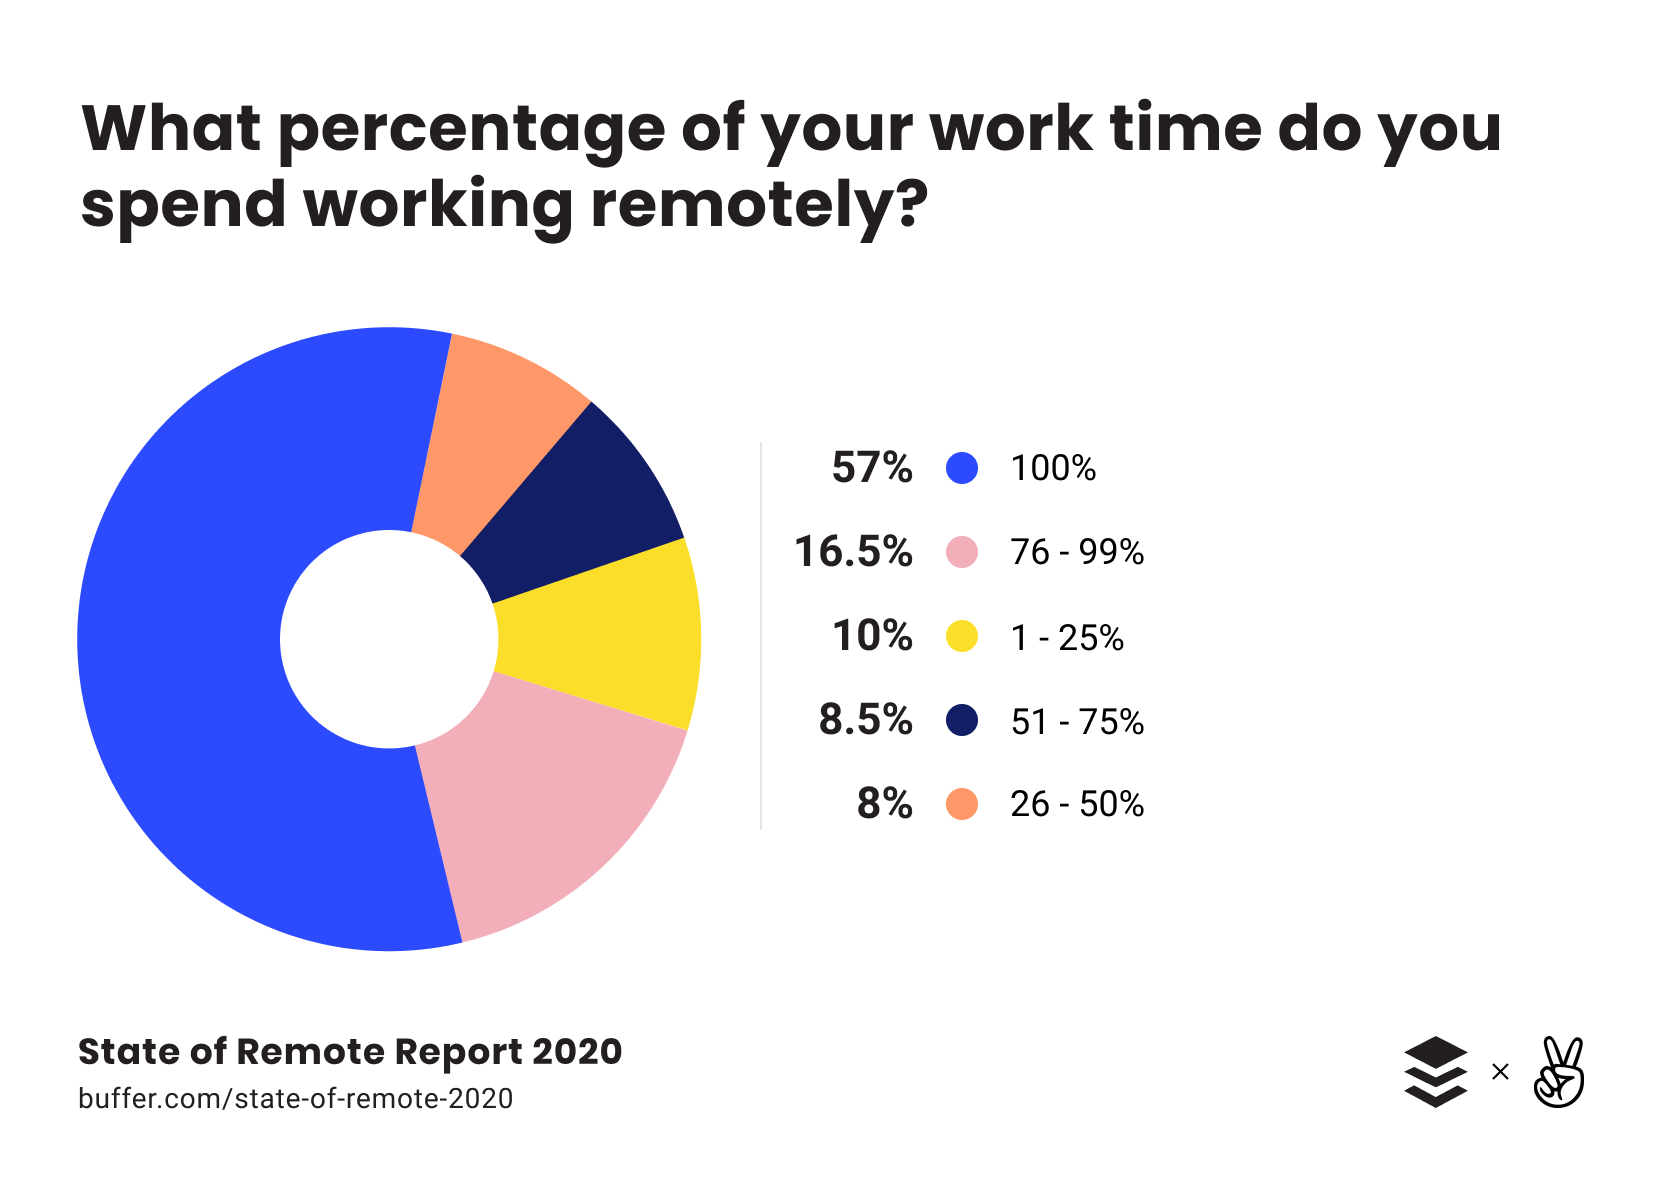
\includegraphics[width=\textwidth]{chart3.png} 
\caption{Percentage of Time Spent Working Remotely (Source: https://buffer.com/state-of-remote-work/2020)}
\end{figure}

The above graph is a Pie Graph showing percentage of work time spent working remotely. This graph displays this data with different colors representing percentages of working remote ranging from 100\% to 1\%. 

\pagebreak 

\section{Audience and action suitability}
\subsubsection{Visualization 1}
The fertility rate graph doesn’t display a strong action the user should take but rather tries to inform the user in the best way possible, which it does very well. This graph is presented in way that highlights no specific target audience, making it effective in communicating data to the general population, rather than a specific demographic. This graph also presents as a trust worthy piece of information rather than a 'flashy' infographic, suggesting that it would most likely be used in reports and research papers. The type of graph used, a line graph, also works well for the timeseries data and showing different income brackets, making the graph clear, easy to read and easy to comprehend. 

\subsubsection{Visualization 2}
The Work Remotely graph is a very simple graph showing a single statistic, the percentage of work done remotely. Although, overall this graph does not display the intended data in a clear, comprehensive or effective way. The graph is slightly confusing to follow with the legend being arguably in the wrong order when paired with the chart.  The graph type, a Pie chart, is the correct way to go when it comes to these percentages however its not effective when paired with the legend and the graph itself becomes unnecessary when nested with the legend.


\section{Critical evaluation of structure}
\subsubsection{Visualization 1}
The Fertility Rate graph looks very informative, but on closer inspection, its missing data would provide a clearer picture and more informative graph. Such data includes what constitutes a “Low-income” Country or any of the income brackets, and what countries fall into what income bracket? The graph, being a line graph with multiple colors of lines, is a very effective way of showing this time series data of multiple data groups. The plot structure is clear with none of the graphs being hard to read or interpret, the legend being color coded and aligned to the lines makes it extremely clear with no confusion. The line colors for “World” and “High Income Countries" could be confused but they do not overlap nor come close together, so this is not an issue with the aligned legend to the lines. Overall, the graph is well structured with no confusion on any of the data trying to be presented, apart from the small amount of missing information that would help with context of the graphs data, this graph is comprehensive and informative.

\subsubsection{Visualization 2}
When looking at the Work Remotely graph, it’s a very simple graph, however it doesn’t display the information effectively. The graph and legend do not work together, if the Pie plot was removed and only the legend was present no data would be lost which is an ineffective use of the plot. The Pie Plot Type is however the best for this type of percentage data. The legend is also in wrong order, the legend is in order from highest percentage to lowest of people in each group, this is ineffective as that graph is meant to represent this data not the legend and to have the legend centered around this data make the legend confusing to read. The plot colors also don’t match the order of the legend, this makes it difficult to find the information quickly. Overall, the graph is laid out incorrectly making data difficult to make out at a quick glance.


\section{Critical evaluation of aesthetic choices}
\subsubsection{Visualization 1}
The Fertility Rate graph’s aesthetics are clean and well thought out, the data is not cramped and well spread out, the only coloring is to represent the different groupings, and this is very effective. No unnecessary space used or taken up by non-important information. 

\subsubsection{Visualization 2}
The Work remotely graph’s aesthetics are 'harsh', empty space top the right of the graph and the wrong information is bold in the legend. The colours, however, do make it easy to distinguish the different groupings. The plot itself also has lots of space inside the segments going unused.+


\section{Recommendations}
\subsubsection{Visualization 1}
For the Fertility Rate graph the 1st improvement would be the additional information about the groupings on how they are defined and maybe what countries are in them, this would make the graph have more context and be more useable. The 2nd recommendation would be vertical lines from top to bottom indicating each decade as it could be hard to determine what year the data is at, at the top of the plot. A 3rd recommendation would be to have more distinct colors for each grouping line, this is because as is the graph was to be extrapolated the lines could cross and get closer together and this could lead to groupings getting confused with each other. 

\subsubsection{Visualization 2}
For the Work remotely graph the 1st recommendation would be to better use the space, place the Pie percentages around or inside the Pie Graph itself, this would make the plot useful and have a purpose. 2nd improvement is to reorder the legend and plot as it should be ordered in terms of work percentage this is also how the plot should be ordered clockwise, this is for better readability. 3rd recommendation is the layout, to the right of the graph there is a lot of empty space. Balancing the graph out and would make it more pleasing to look at, in addition to the graph being centered and cropped to reduce empty space. 

\end{document}